\documentclass[../main.tex]{subfiles}


\begin{document}



\tikzset{every picture/.style={line width=0.75pt}} %set default line width to 0.75pt        

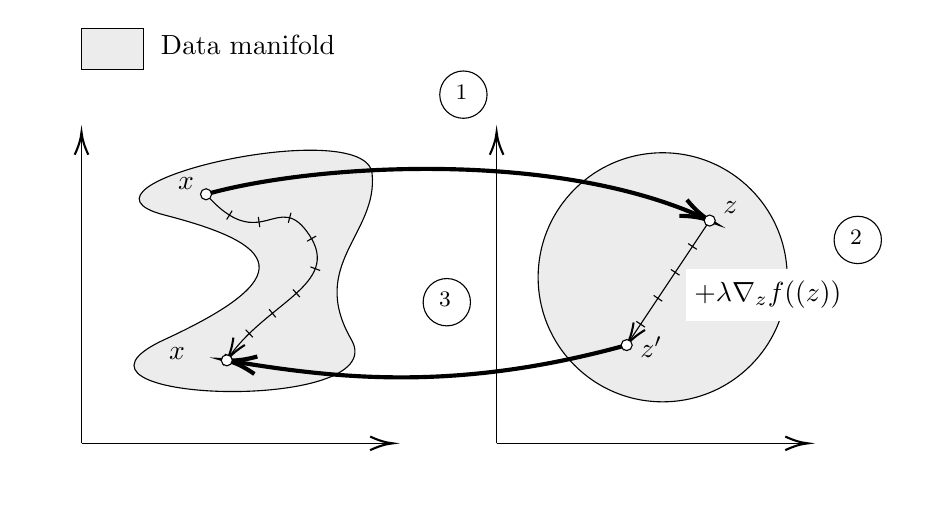
\begin{tikzpicture}[x=0.75pt,y=0.75pt,yscale=-1,xscale=1]
    %uncomment if require: \path (0,300); %set diagram left start at 0, and has height of 300

    %Straight Lines [id:da11442367734571701] 
    \draw    (100,200) -- (100,52) ;
    \draw [shift={(100,50)}, rotate = 90] [color={rgb, 255:red, 0; green, 0; blue, 0 }  ][line width=0.75]    (10.93,-3.29) .. controls (6.95,-1.4) and (3.31,-0.3) .. (0,0) .. controls (3.31,0.3) and (6.95,1.4) .. (10.93,3.29)   ;
    %Straight Lines [id:da7963766384193337] 
    \draw    (100,200) -- (248,200) ;
    \draw [shift={(250,200)}, rotate = 180] [color={rgb, 255:red, 0; green, 0; blue, 0 }  ][line width=0.75]    (10.93,-3.29) .. controls (6.95,-1.4) and (3.31,-0.3) .. (0,0) .. controls (3.31,0.3) and (6.95,1.4) .. (10.93,3.29)   ;
    %Straight Lines [id:da2658315064564406] 
    \draw    (300,200) -- (300,52) ;
    \draw [shift={(300,50)}, rotate = 90] [color={rgb, 255:red, 0; green, 0; blue, 0 }  ][line width=0.75]    (10.93,-3.29) .. controls (6.95,-1.4) and (3.31,-0.3) .. (0,0) .. controls (3.31,0.3) and (6.95,1.4) .. (10.93,3.29)   ;
    %Straight Lines [id:da18089884074200846] 
    \draw    (300,200) -- (448,200) ;
    \draw [shift={(450,200)}, rotate = 180] [color={rgb, 255:red, 0; green, 0; blue, 0 }  ][line width=0.75]    (10.93,-3.29) .. controls (6.95,-1.4) and (3.31,-0.3) .. (0,0) .. controls (3.31,0.3) and (6.95,1.4) .. (10.93,3.29)   ;
    %Shape: Polygon Curved [id:ds8536523285813445] 
    \draw  [fill={rgb, 255:red, 155; green, 155; blue, 155 }  ,fill opacity=0.19 ] (140,90) .. controls (84.33,75.67) and (237,41) .. (240,70) .. controls (243,99) and (209,113.67) .. (230,150) .. controls (251,186.33) and (74.33,180.33) .. (140,150) .. controls (205.67,119.67) and (195.67,104.33) .. (140,90) -- cycle ;
    %Shape: Circle [id:dp37911959920066995] 
    \draw  [fill={rgb, 255:red, 155; green, 155; blue, 155 }  ,fill opacity=0.19 ] (320,120) .. controls (320,86.86) and (346.86,60) .. (380,60) .. controls (413.14,60) and (440,86.86) .. (440,120) .. controls (440,153.14) and (413.14,180) .. (380,180) .. controls (346.86,180) and (320,153.14) .. (320,120) -- cycle ;
    %Shape: Rectangle [id:dp7322085910834354] 
    \draw  [fill={rgb, 255:red, 155; green, 155; blue, 155 }  ,fill opacity=0.19 ] (100,0) -- (130,0) -- (130,20) -- (100,20) -- cycle ;
    %Curve Lines [id:da8575381600409676] 
    \draw [line width=1.5]    (160,80) .. controls (211.15,65.48) and (327.97,58.15) .. (400.48,91.64) ;
    \draw [shift={(402.67,92.67)}, rotate = 205.61] [color={rgb, 255:red, 0; green, 0; blue, 0 }  ][line width=1.5]    (14.21,-4.28) .. controls (9.04,-1.82) and (4.3,-0.39) .. (0,0) .. controls (4.3,0.39) and (9.04,1.82) .. (14.21,4.28)   ;
    %Straight Lines [id:da18727578769657827] 
    \draw    (402.67,92.67) -- (363.78,151) (396.43,106.53) -- (392.27,103.76)(388.11,119.01) -- (383.95,116.24)(379.79,131.5) -- (375.63,128.72)(371.46,143.98) -- (367.3,141.2) ;
    \draw [shift={(362.67,152.67)}, rotate = 303.69] [color={rgb, 255:red, 0; green, 0; blue, 0 }  ][line width=0.75]    (10.93,-3.29) .. controls (6.95,-1.4) and (3.31,-0.3) .. (0,0) .. controls (3.31,0.3) and (6.95,1.4) .. (10.93,3.29)   ;
    %Shape: Circle [id:dp738703397178804] 
    \draw  [fill={rgb, 255:red, 255; green, 255; blue, 255 }  ,fill opacity=1 ] (400,92.67) .. controls (400,91.19) and (401.19,90) .. (402.67,90) .. controls (404.14,90) and (405.33,91.19) .. (405.33,92.67) .. controls (405.33,94.14) and (404.14,95.33) .. (402.67,95.33) .. controls (401.19,95.33) and (400,94.14) .. (400,92.67) -- cycle ;
    %Curve Lines [id:da944586344717079] 
    \draw [line width=1.5]    (173.24,160.55) .. controls (226.29,169.4) and (282.63,174.72) .. (362.67,152.67) ;
    \draw [shift={(170,160)}, rotate = 9.63] [color={rgb, 255:red, 0; green, 0; blue, 0 }  ][line width=1.5]    (14.21,-4.28) .. controls (9.04,-1.82) and (4.3,-0.39) .. (0,0) .. controls (4.3,0.39) and (9.04,1.82) .. (14.21,4.28)   ;
    %Shape: Circle [id:dp47523071366663894] 
    \draw  [fill={rgb, 255:red, 255; green, 255; blue, 255 }  ,fill opacity=1 ] (360,152.67) .. controls (360,151.19) and (361.19,150) .. (362.67,150) .. controls (364.14,150) and (365.33,151.19) .. (365.33,152.67) .. controls (365.33,154.14) and (364.14,155.33) .. (362.67,155.33) .. controls (361.19,155.33) and (360,154.14) .. (360,152.67) -- cycle ;
    %Curve Lines [id:da8730458701921838] 
    \draw    (160,80) .. controls (187,110.71) and (194.6,76.2) .. (210,100) .. controls (225.09,123.32) and (189.11,132.4) .. (171.08,158.39)(172.58,87.92) -- (169.94,92.16)(185.19,90.89) -- (185.88,95.84)(200.92,88.91) -- (199.64,93.75)(213.01,100.14) -- (208.68,102.63)(214.97,116.73) -- (210.29,114.97)(205.21,129.53) -- (201.83,125.84)(193.56,139.27) -- (190.4,135.4)(182.57,148.88) -- (179.09,145.29)(173.13,159.81) -- (169.03,156.96) ;
    \draw [shift={(170,160)}, rotate = 302.9] [color={rgb, 255:red, 0; green, 0; blue, 0 }  ][line width=0.75]    (10.93,-3.29) .. controls (6.95,-1.4) and (3.31,-0.3) .. (0,0) .. controls (3.31,0.3) and (6.95,1.4) .. (10.93,3.29)   ;
    %Shape: Circle [id:dp4115107343777302] 
    \draw  [fill={rgb, 255:red, 255; green, 255; blue, 255 }  ,fill opacity=1 ] (167.33,160) .. controls (167.33,158.53) and (168.53,157.33) .. (170,157.33) .. controls (171.47,157.33) and (172.67,158.53) .. (172.67,160) .. controls (172.67,161.47) and (171.47,162.67) .. (170,162.67) .. controls (168.53,162.67) and (167.33,161.47) .. (167.33,160) -- cycle ;
    %Shape: Circle [id:dp48922593926577407] 
    \draw  [fill={rgb, 255:red, 255; green, 255; blue, 255 }  ,fill opacity=1 ] (157.33,80) .. controls (157.33,78.53) and (158.53,77.33) .. (160,77.33) .. controls (161.47,77.33) and (162.67,78.53) .. (162.67,80) .. controls (162.67,81.47) and (161.47,82.67) .. (160,82.67) .. controls (158.53,82.67) and (157.33,81.47) .. (157.33,80) -- cycle ;

    % Text Node
    \draw (137,2) node [anchor=north west][inner sep=0.75pt]   [align=left] {Data manifold};
    % Text Node
    \draw (145.33,70.73) node [anchor=north west][inner sep=0.75pt]    {$x$};
    % Text Node
    \draw (408,82.4) node [anchor=north west][inner sep=0.75pt]    {$z$};
    % Text Node
    \draw (368,147.4) node [anchor=north west][inner sep=0.75pt]    {$z'$};
    % Text Node
    \draw (251,46.4) node [anchor=north west][inner sep=0.75pt]    {$\enc$};
    % Text Node
    \draw (141,152.4) node [anchor=north west][inner sep=0.75pt]    {$\CF{x}$};
    % Text Node
    \draw (241,147.4) node [anchor=north west][inner sep=0.75pt]    {$\dec$};
    % Text Node
    \draw  [draw opacity=0][fill={rgb, 255:red, 255; green, 255; blue, 255 }  ,fill opacity=1 ]  (391,116) -- (496,116) -- (496,141) -- (391,141) -- cycle  ;
    \draw (394,120.4) node [anchor=north west][inner sep=0.75pt]    {$+\lambda \nabla_{z} f(\dec(z))$};
    % Text Node
    \draw    (276, 132) circle [x radius= 11.4, y radius= 11.4]   ;
    \draw (271,126) node [anchor=north west][inner sep=0.75pt]  [font=\footnotesize] [align=left] {3};
    % Text Node
    \draw    (474, 102) circle [x radius= 11.4, y radius= 11.4]   ;
    \draw (469,96) node [anchor=north west][inner sep=0.75pt]  [font=\footnotesize] [align=left] {2};
    % Text Node
    \draw    (284, 32) circle [x radius= 11.4, y radius= 11.4]   ;
    \draw (279,26) node [anchor=north west][inner sep=0.75pt]  [font=\footnotesize] [align=left] {1};
    % Text Node
    \draw (174.5,215) node   [align=left] {\begin{minipage}[lt]{68pt}\setlength\topsep{0pt}
            \begin{center}
                $\displaystyle \inputspace$
            \end{center}

        \end{minipage}};
    % Text Node
    \draw (375.5,215) node   [align=left] {\begin{minipage}[lt]{68pt}\setlength\topsep{0pt}
            \begin{center}
                $\displaystyle \latentspace$
            \end{center}

        \end{minipage}};


\end{tikzpicture}



\end{document}